%%%%%%%%%%%%%%%%%%%%%%%%%%%%%%%%%%%%%%%
% 3.1: proximal operator
% definitions, basics and algorithm
%%%%%%%%%%%%%%%%%%%%%%%%%%%%%%%%%%%%%%%

\subsection{Compute the proximal operator}

In many cases, to improve the computation cost of a function $f$, we consider the proximal mapping. Fast algorithm already exist to compute these objects such as FISTA \cite{beck2009fast}, the proximal gradient method \cite{ryu2017proximal}, \dots

% proximal operator
\begin{definition}[Moreau's proximal mapping]\label{def:prox}
Let $f$ be a real function, its proximal operator (or Moreau's proximal operator) $\prox_f$ is defined as follows:
\[\forall x\in\EE,\ \prox_f(x) =\arg\min_{u\in \EE}\left\{f(u) + \frac{1}{2}\|u-x\|^2_2\right\}\enspace.\] 
\end{definition}

This can be either a set of multiple elements, an empty set or a singleton. In our case, the following lemma and theorem assure that $\abs{\prox_{\mathcal{S}(x)}} = 1$. The proof is available in \cite{beck}.

% S_k is closed => needed for the singleton of prox
\begin{lemma}
The sparse envelope $\mathcal{S}_k$ is closed \emph{ie} for all $y \in \RR,\ \left\{x\in \mathcal{D}_f\, |\, f(x)\leq y\right\}$ is closed.
\end{lemma}
\begin{theorem}\label{thm:unicityprox}
For a proper closed convex function $f$, $\abs{\prox_f(x)} = 1$ for all $x\in\EE$.
\end{theorem}

When solving an inverse problem, as we saw with the ridge penalty or \enet, there is an hyperparameter multiplying the penalty factor. Let's note it $\lambda_s>0$ for the sparse envelope. Then \ref{thm:unicityprox} still holds and there is an almost explicit formulation for the value of $\prox_{\lambda\mathcal{S}_k}$.

% form for the \lambda prox_k(x) with u_i 
\begin{proposition}
From $u=\min\limits_{u\in D_k}\sum_{i=1}^n \phi(x_i,\lambda + u_i)$ with $\lambda > 0$, we can compute $w=\prox_{\lambda\mathcal{S}_k}(x)$ defined as:
\begin{equation}\label{eq:proxui}
    \forall\ i=1,\dots,n\ w_i=\frac{x_iu_i}{\lambda + u_i}\enspace.
\end{equation}
\end{proposition}
\begin{proof}
Using definition \ref{def:prox} followed by proposition \ref{prop:Sfromphi}, \[\begin{aligned}
w&=\arg\min_{z\in\RR^n}\left\{\lambda\mathcal{S}_k(z) + \frac{1}{2}\|z-x\|^2_2\right\} = \arg\min_{z\in\RR^n}\left\{\frac{\lambda}{2}\min_{u\in D_k}\sum_{i=1}^n\phi(z_i, u_i) + \frac{1}{2}\|z-x\|^2_2\right\}\\
&=\arg\min_{z\in\RR^n}\min_{u\in D_k}\underbrace{\left\{\frac{\lambda}{2}\sum_{i=1}^n\phi(z_i, u_i) + \frac{1}{2}\|z-x\|^2_2\right\}}_{\varphi}\enspace.
\end{aligned}\]
From there, we need to solve for $z$ the inner minimization. We note $\hat z$ the value at the optimum. Suppose that $u_i>0$ (otherwise $u_i=0=\hat z_i$), then from the first order condition for all $i_0=1,\dots,n$:
\[\begin{aligned}
\frac{\partial\varphi}{\partial z_{i_0}}(x, \hat z, u)= 0 &\Longleftrightarrow \frac{\lambda}{2}\frac{2\hat z_{i_0}}{u_{i_0}} + \frac{2}{2}(\hat z_{i_0} - u_{i_0})\\
& \Longleftrightarrow \hat z_{i_0} = \frac{u_{i_0}z_{i_0}}{\lambda + u_{i_0}}\enspace.
\end{aligned}\]
And plugging-in this result, it is easy to show that $\varphi(x,\hat z, u) = \frac{\lambda}{2}\sum_{i=1}^n \phi(x_i, \lambda + u_i)$.
\end{proof}

%%%%%%%%%%%%%%%%%%%%%%%%%%%%%%%%%%
% Algorithm to compute SE
%%%%%%%%%%%%%%%%%%%%%%%%%%%%%%%%%%
\subsection[Algorithm]{Algorithms for the sparse envelope}
To find the root of a function defined as the sum of piecewise linear functions with a single breakpoint, we can use the \textit{Random Search} algorithm.
\begin{figure}[H]
    \center
    
    \begin{tikzpicture}[node distance=1.5cm,
        every node/.style={fill=white, font=\sffamily}, align=center]
      % Specification of nodes (position, etc.)
      \node (start)[ activityStarts]{Input: $\alpha^2,\alpha^2, \beta^1 \beta^2\in \RR^n, \delta\in\RR$\\ $F=\sum_{i=1}^nF_j - \delta$};
      \node (beginning)[process, below of=start]{
      Init: $\Omega = \{1,\dots,n\}$\\ $\tilde\alpha=0$, $\tilde\beta=0$};
      \node (while)[process, below of=beginning]{
      While $\Omega\neq\emptyset$:\\
      Pick randomly $p\in\Omega$\\
      $F(\gamma_p)\leftarrow \tilde\alpha\gamma_p + \tilde\beta + \sum_{j\in\Omega}F_j(\gamma_p)$};
      \node(pos)[process, below of=while, yshift=-1.5cm, xshift=-4cm]{
      If $F(\gamma_p)>0$:\\
      $A\leftarrow \{j\in\Omega\,|\, \gamma_j<\gamma_p\}$\\
      $\tilde\alpha\leftarrow \tilde\alpha + \sum_{j\in\Omega\setminus A}\alpha_j^1$\\
      $\tilde\beta \leftarrow \tilde\beta + \sum_{j\in \Omega\setminus A}\beta_j^1$\\
      $\Omega\leftarrow A$};
      \node(neg)[process, below of=while, yshift=-1.5cm, xshift=+4cm]{
      If $F(\gamma_p)<0$:\\
      $A\leftarrow \{j\in\Omega\,|\, \gamma_j>\gamma_p\}$\\
      $\tilde\alpha\leftarrow \tilde\alpha + \sum_{j\in\Omega\setminus A}\alpha_j^2$\\
      $\tilde\beta \leftarrow \tilde\beta + \sum_{j\in \Omega\setminus A}\beta_j^2$\\
      $\Omega\leftarrow A$};
      \node(end0)[startstop, below of=while, yshift=-1.5cm]{If $F(\gamma_p)=0$:\\ \textbf{Return}: $\eta^*=\gamma_p$};
      \node(endwhile)[startstop, below of=end0, yshift=-.7cm]{
      \textbf{Return:} $\eta^*=-\tilde\beta / \tilde\alpha$};
      
      % draw the lined
      \draw[->] (start)   --  (beginning);
      \draw[->] (beginning)   --  (while);
      \draw[->] (while) -- (pos);
      \draw[->] (while) -- (neg);
      \draw[->, dotted, line width=2pt] (pos) --++ (0,3) --++ (while);
      \draw[->, dotted, line width=2pt] (neg) --++ (0,3) --++ (while);
      \draw[->] (while) -- (end0);
      \draw[->] (while.north west) --++(3,0) -- node[right]{If $\Omega=\emptyset$} ++(6,0) |- (endwhile);
    
      \end{tikzpicture}
      
      \label{fig:algorand}
      \caption{Diagram for the random search algorithm procedure.}
      
    \end{figure}

\begin{remark}
Note that this algorithm exploits the fact that the problem was reduced from finding a vector of dimension $n$ to finding the root of a function in one dimension. Besides, it is efficient with sparse vectors because of the choice of the $F_j$ functions in the sum. In the worse case, we find ourselves with a complexity of $\mathcal{O}(n)$ that does not depend on the size of an initial interval like the bisection method.
\end{remark}

% figure for decomposition into sum of single-breakpoints
\begin{figure}[H]
    \centering
    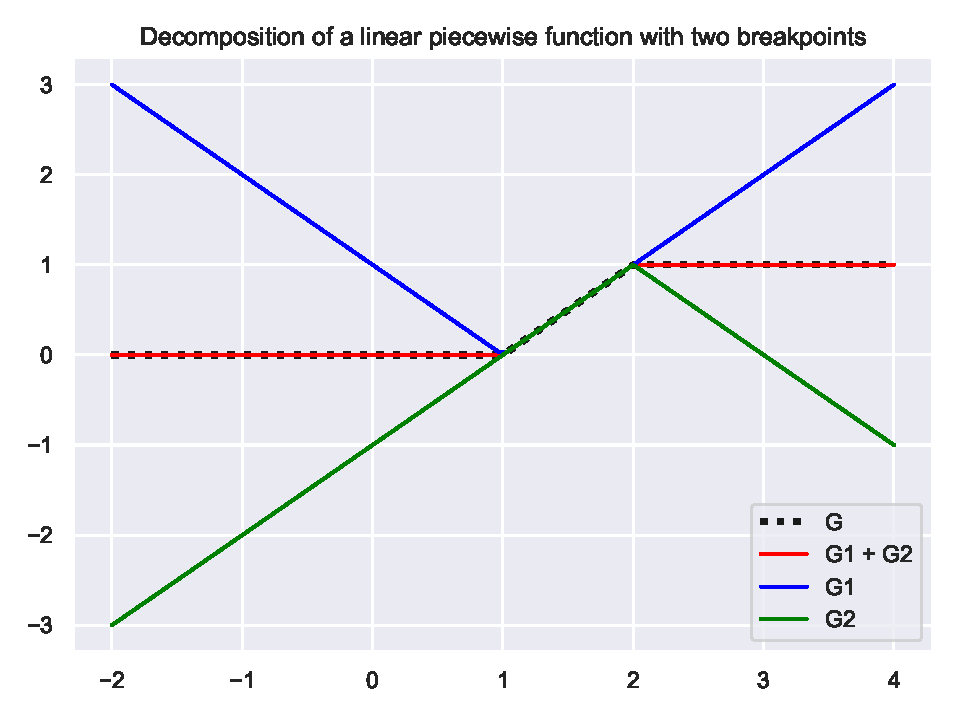
\includegraphics[height=6cm, trim={0cm 0Cm 0cm 1cm}, clip]{images/decomposition.pdf}
    \caption{Decomposition of a piecewise linear signal with two breakpoints into the sum of two piecewise learn signals with a single breakpoint each.}
    \label{fig:decomposition}
\end{figure}

%%%%%%%%%%%%%%%%%%%%%%%%%%%%%%%%%%
% Numerical results part : 
%%%%%%%%%%%%%%%%%%%%%%%%%%%%%%%%%%
\subsection{Numerical application}

Let's finally compare our regularized problem with the \enet
regularization in an highly correlated situation (the same represented in Figure \ref{fig:lasso_enet}).
We simulate a signal with only $3$'s for the first fifteen components and zeros for the $25$ left. The observed signal is 
\[ b = Ax + \varepsilon\enspace,\]
where $\varepsilon\sim\mathcal{N}(0,\sigma^2)$ is a Gaussian noise.
The matrix $A$ is constructed from the algorithm that follows so that we can recreate the grouping effect:
\begin{itemize}
\setlength{\arraycolsep}{1pt} % resize matrices
    \item generate three random vectors $z_1,\ z_2$ and $z_3\in\RR^n$,
    \item from $z_i$, compute $Z_i=\begin{bmatrix} z_i, & z_i, & z_i, & z_i, & z_i\end{bmatrix}\in\RR^{n\times 5}$,
    \item generate $B,\ C,\ D\in\RR^{n\times 5}$ and $E\in\RR^{n\times 25}$,
    \item $A=\begin{bmatrix}Z_1 + 0.01 W_1, & Z_2 + 0.01 W_2, & Z_3 + 0.01 W_3, & E \end{bmatrix}$.
\end{itemize}

%%%%%%%%%%% End the data preparation %%%%%%%%%%%%%
%%%%%%%%%%% Begin numerical analysis %%%%%%%%%%%%%

The sparse-envelope problem is written as:
\[\min_{x\in \RR^n} \|Ax-b\|^2_2 + \lambda\mathcal{S}_k(x)\enspace,\]
where $\lambda$ must be chosen through a train/test procedure and we take $k=15$ because we know its real value here. Otherwise we would have to search it as well.

% Figure enet and prox signal together
\begin{center}
    \begin{figure}[H]
        \centering
        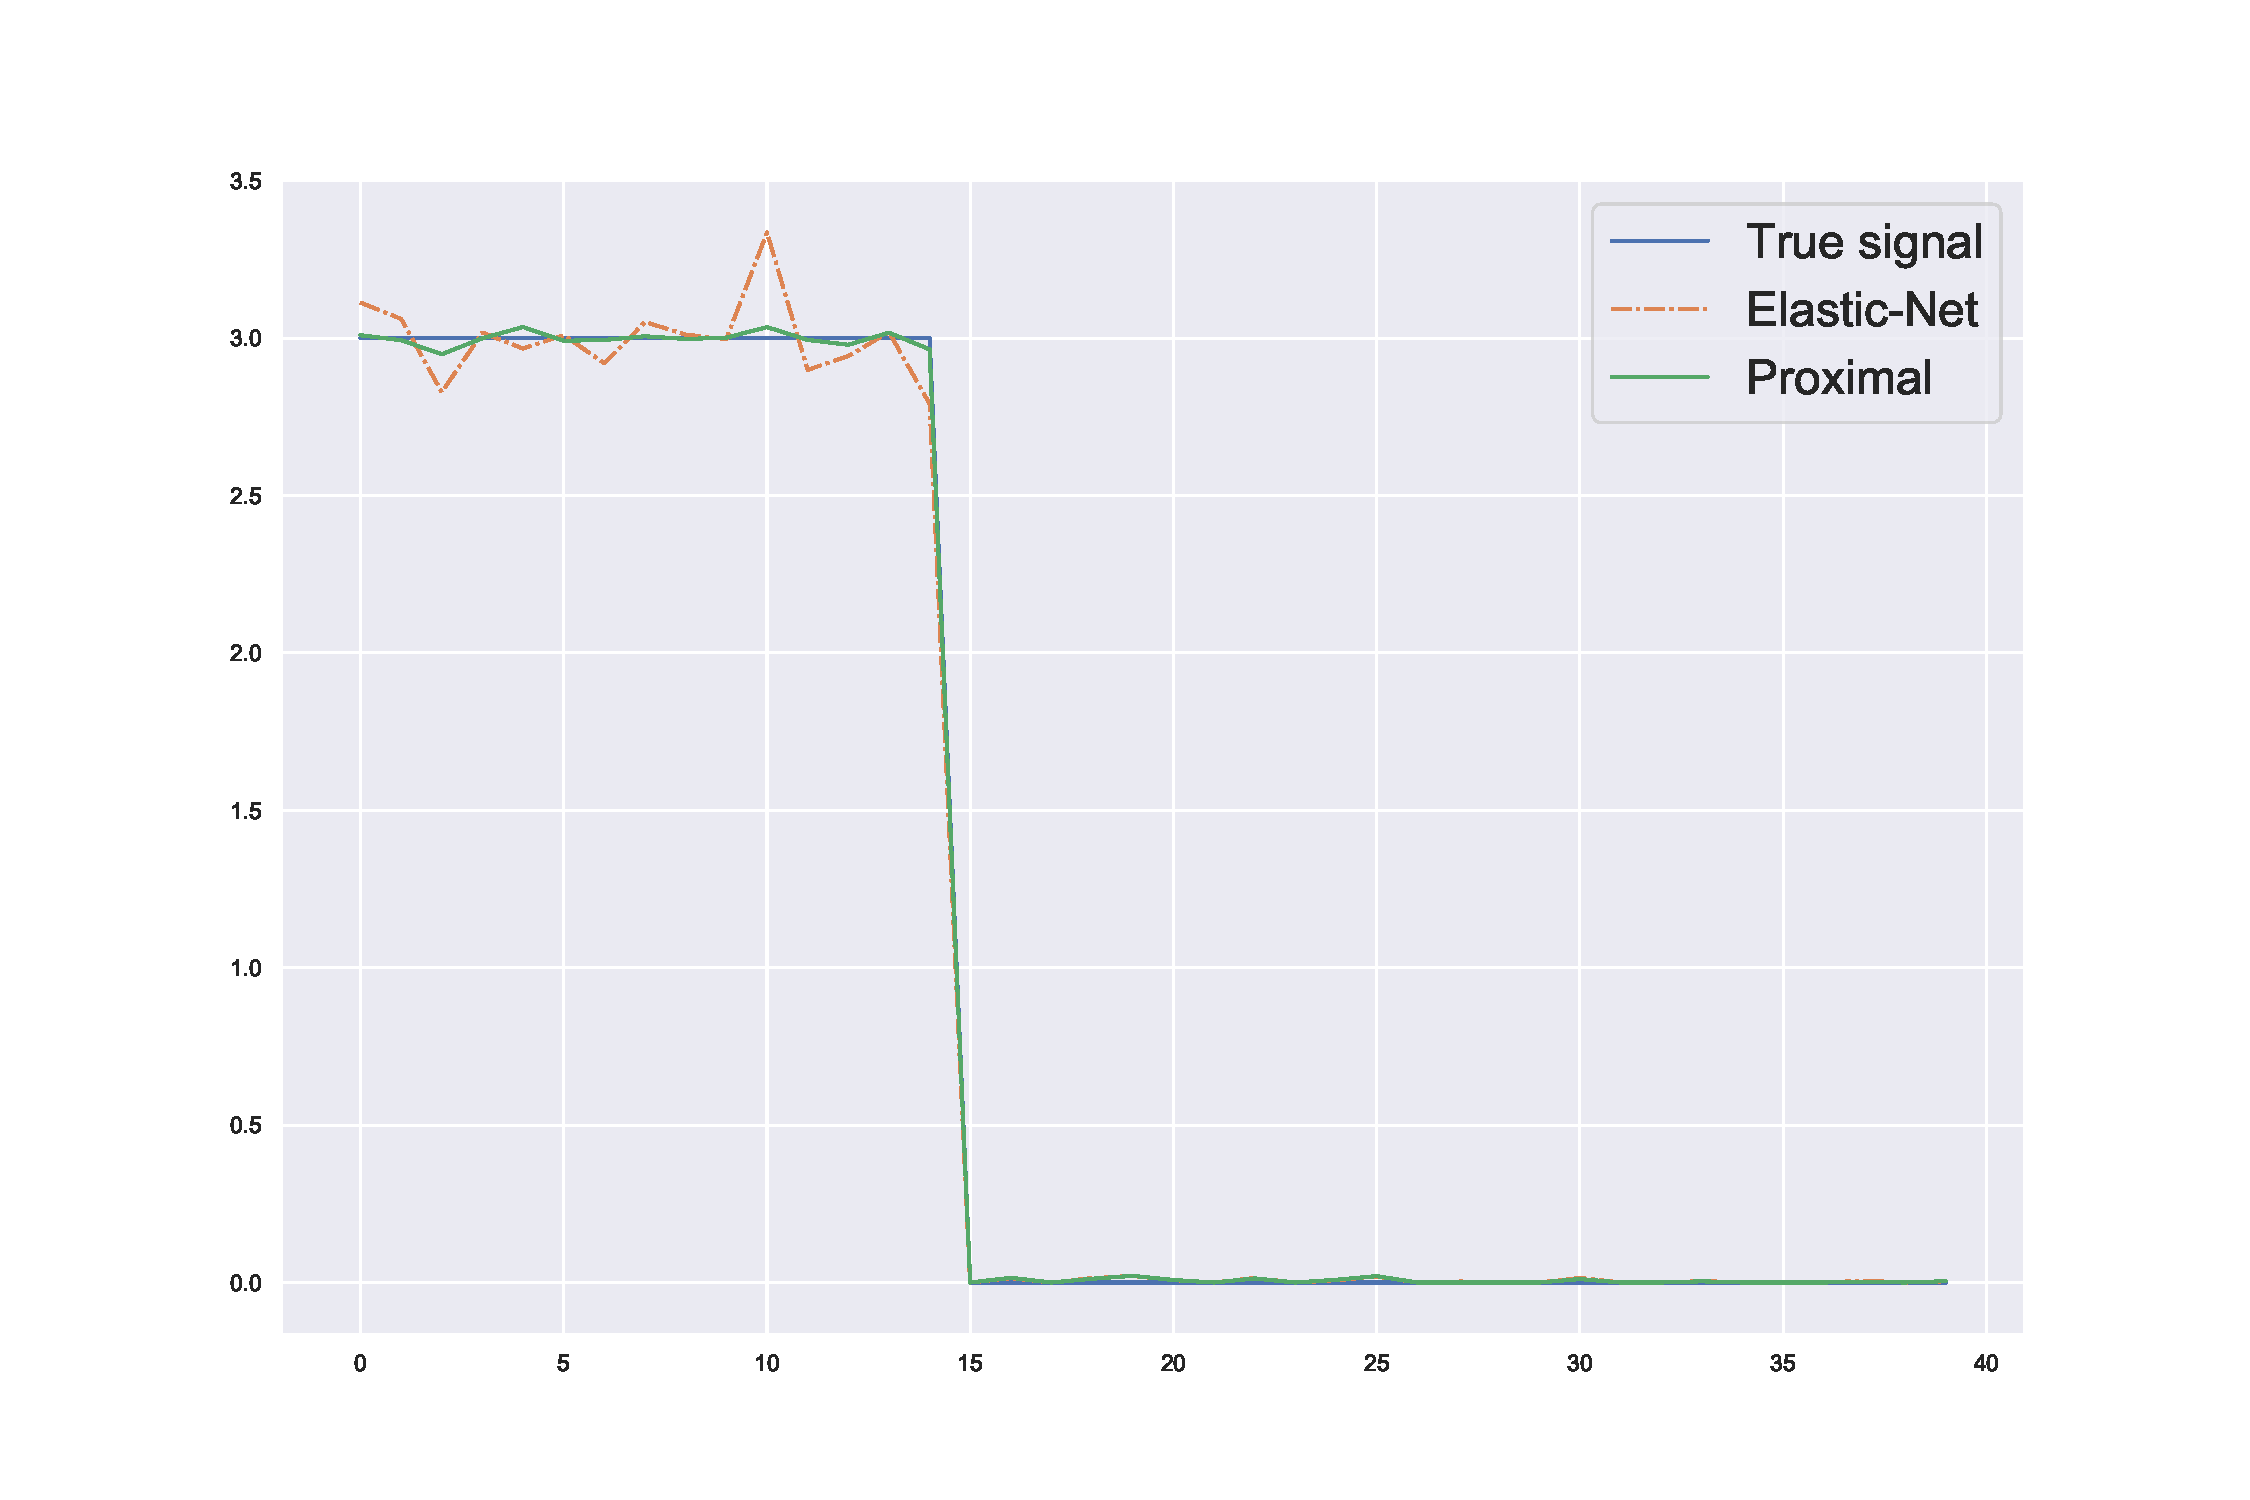
\includegraphics[width=.9\linewidth]{images/enet_proxi.pdf}
        \caption{Comparison of the Elastic-net and sparse regularization in a highly correlated situation with $n=50$ and $\sigma=0.1$.}
        \label{fig:enet_sp}
    \end{figure}
\end{center}

As the Figure \ref{fig:enet_sp} shows, the proximal envelope is closer to the original signal than the \enet in this case.
We can now compare if this is also the case for some values of $n\in\NN^*$ and quantify the gain of using this method instead of the \enet currently used.

\paragraph*{}
%% Table of the results for the diminution of the residuals
To do so, we call $x_{enet}$ the solution returned by the \enet method and $x_{prox}$ the one returned by the method we described. The residuals are respectively $\|x-x_{enet}\|_2$ and $\|x-x_{prox}\|_2$ for both methods. Finally, we want to look at the improvement made by the latter against the former. So the percentage of improvement of the residuals is given by:
\[\mathrm{IM}(x_{prox}\,||\,x_{enet})=\left(\frac{\|x-x_{prox}\|_2}{\|x-x_{enet}\|_2} - 1 \right) \times 100\enspace.\]

To see different cases, we tried $n\in\{40, 80\}$ and $\sigma\in\{0.1,1,2\}$.
We generated new data for $A$ (and therefore $b$) $J=50$ times for each experiment, the improvements percentages showed are defined as
\[\bar{\mathrm{IM}}_{n}(J) = \frac{1}{J}\sum_{j=1}^J \mathrm{IM}(x_{prox}^{(j)}\,||\, x_{enet}^{(j)})\enspace.\]

\begin{remark}
A negative improvement in this case means that the error was reduced from the \enet to the sparse envelope method. If the sparse envelope method were perfect and resulted in $x=x_{prox}$, then $\mathrm{IM}(x_{prox}\,||x_{enet})=-100\%$. \end{remark}

In addition to the mean of the improvements, we provide the standard deviation needed for the confidence interval (each simulation is indeed independent of the previous ones and we generate the data with normal distributions of fixed parameters for a chosen $\sigma$).

% results table: SE way better in this case
\begin{table}[H]
    \centering
    \begin{tabular}{cccc}
    $n$ & $\sigma$ & $\bar{\mathrm{IM}}_n(50)$ & $\hat\sigma\left(\mathrm{IM}_n(50)\right)$\\
    \hline
    $40$     &  $0.1$ & $-98.55\%$ & $0.510$ \\
             &  $1.0$ & $-98.29\%$ & $0.543$\\
             &  $2.0$ & $-97.75\%$ & $0.768$\\  \hline
    $80$     &  $0.1$ & $-99.09\%$ & $0.308$\\
             &  $1.0$ & $-99.15\%$ & $0.361$\\
             &  $2.0$ & $-98.79\%$ & $0.580$\\
    \end{tabular}
    \caption{Average improvement obtained comparing for the residuals of the inverse problem using the \enet method against the sparse envelope.}
    \label{tab:endresults}
\end{table}

From Table \ref{tab:endresults} and Figure \ref{fig:enet_sp}, we can conclude that in situations involving a grouping effect, the sparse envelope has a better accuracy than the \enet. However, the bigger the noise, the closer the two method get (especially on the part of the signal where the true signal equals zero). 
